% This file is isea.tex.  It contains the formatting instructions for and acts as a template for submissions to ISEA 2015.  It is based on the ICCC  formats and instructions.  It uses the files isea.sty, isea.bst and isea.bib, the first two of which also borrow from AAAI IJCAI formats and instructions.
% Modified from ICCC.tex by B. Bogart

\documentclass[letterpaper]{article}
\usepackage{isea}
\usepackage[pdftex]{graphicx}
\usepackage{times}
\usepackage{helvet}
\usepackage{courier}
\usepackage[numbers]{natbib}
\pdfinfo{
/Title (Accelerating XDP Programs Using HW-based Hints)
/Author (Peter P. Waskiewicz Jr)}
% The file isea.sty is the style file for ISEA 2015 proceedings.
%
\title{Accelerating XDP Programs Using HW-based Hints}
\author{Peter P. Waskiewicz Jr. \\ Intel \\ Hillsboro, OR, USA \\ peter.waskiewicz.jr@intel.com
\And Anjali Singhai Jain \\ Intel \\ Hillsboro, OR, USA \\ anjali.singhai@intel.com
\And Neerav Parikh \\ Intel \\ Hillsboro, OR, USA \\ neerav.parikh@intel.com
\And Parthasarathy Sarangam \\ Intel \\ Hillsboro, OR, USA \\ parthasarathy.sarangam@intel.com
\newline
\newline
}
\setcounter{secnumdepth}{0}

\begin{document} 
\maketitle
\begin{abstract}
As XDP workloads continue to evolve, they are becoming more complex.  They can parse deeper into a packet to make more complex decisions, plus they may compute more complex hashing or other CPU-intensive operations to make flow-based decisions.

This talk will focus on efforts to extend the XDP framework to pass HW-based hints that have been computed by the underlying network device.  The intent is to build a framework that is vendor agnostic, so XDP programs don't need to comprehend the underlying device they're running against.

This talk also aims to show a proposed direction for the changes in XDP, along with the proposed additional metadata structure.  It will also show benchmarks of certain XDP workloads with and without HW-based hints, highlighting the benefits of using these existing offloads.
\end{abstract}

\section{Keywords}

networking, kernel, ebpf, xdp, offloads

\section{Introduction}
XDP has already provided a giant leap forward in performance and efficiency for packet processing in Linux. To continue making progress, the eBPF and XDP infrastructure needs to start utilizing existing hardware offloads from a network device. This will reduce computational cycles when parsing packet headers and data, leading to more efficient eBPF and XDP programs. This progress though requires changes to the Linux kernel and surrounding eBPF infrastructure.
\newline
\newline
This paper will focus on proposed changes to eBPF and XDP for the following:
\begin{itemize}
\item Utilize HW-based offloads from a network device driver to provide hints for accelerating XDP programs
\item Share performance metrics from proof-of-concept patches highlighting the acceleration benefits of using HW hints
\item Propose future changes to the eBPF framework in LLVM, clang, and the Linux kernel, to support teaching underlying hardware which hints to provide
\item Propose additional techniques to keep XDP programs vendor-agnostic while still programming desired hints, and then consuming the hints for acceleration
\end{itemize}

\section{HW Offloaded Hints From Device Driver} 

Network hardware already computes a large number of offloads today. Future network hardware, especially with the emergence of SmartNICs \cite{smartnic2016}, will provide even more in terms of offloaded computations. Harnessing this metadata will be crucial to allow more complex eBPF and XDP programs to stay as perfomant as possible.
\newline
\newline
The rest of this paper discusses proposed changes to the XDP core that are built on patches from Daniel Borkman \cite{borkmann2017}, adding a metadata section to the existing xdp\_buff structure in the Linux kernel. Prior to these patches, an xdp\_buff consisted of the following:
\newline
\newline
struct xdp\_buff \{
\newline
\indent{void *data;}
\newline
\indent{void *data\_end;}
\newline
\indent{void *data\_hard\_start;}
\newline
\}
\newline
\newline
After the patches, the structure now looks like this:
\newline
\newline
struct xdp\_buff \{
\newline
\indent{void *data;}
\newline
\indent{void *data\_end;}
\newline
\indent{void *data\_hard\_start;}
\newline
\indent{void *data\_meta;}
\newline
\}
\newline

\begin{figure}[h]
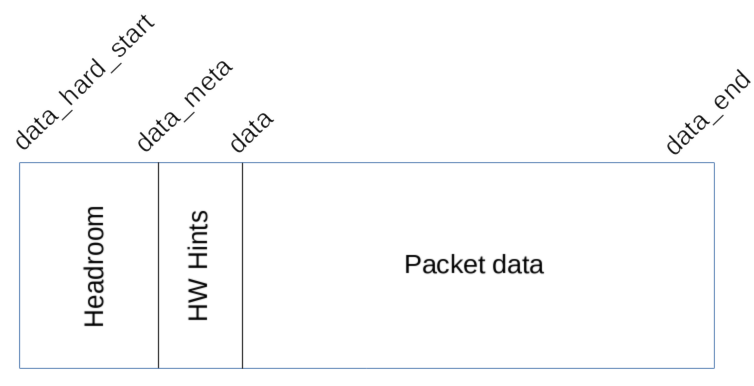
\includegraphics[width=3.31in]{xdp-metadata-layout.png}
\caption{xdp\_buff layout with metadata}
\label{xdp-metadata-layout}
\end{figure}

The new xdp\_buff field, "data\_meta", can be used to point at opaque data sitting inside the headroom in the xdp\_buff memory, prior to the DMA'd packet buffer. This can be seen in Figure \ref{xdp-metadata-layout}. This headroom can then be parsed using proposed eBPF helper functions to extract the HW-based hints from the driver, and then be used in the business logic of the XDP programs.

\subsection{Initial Performance Gains}

Initial performance gains are very promising using HW-based hints. In benchmarks with proof-of-concept patches, where hints are memcpy()'d from the Rx descriptor into the XDP buffer headroom, two XDP programs were used to demonstrate the gains.
\newline
\indent Two programs, XDP3 and XDP\_HINTS, were written to demonstrate the usage of hints. This is compared to the in-kernel XDP1 sample program, designed to parse the packet headers and then drop all traffic.  XDP3 is a copy of XDP1, however it performs no parsing at all. This is to demonstrate the smallest XDP program to take a packet and immediately drop it.  XDP\_HINTS is a modified version of XDP1, where instead of parsing packet data, it consumes metadata from the xdp\_buff provided by the base driver, and then drops the packet. In other words, it performs no packet parsing, but just makes decisions based off metadata.
\newline
\indent Data in Figure \ref {xdp-performance} was collected on an Ivy Bridge-class Xeon platform as the target machine. As seen in the chart, XDP1 with JIT runs at approximately 7.3 million packets/second. XDP3, with no packet parsing but with JIT, runs at approximately 22 million packets/second. XDP\_HINTS, which performs no packet parsing, but uses the HW-provided hints in the XDP metadata, also runs at 22 million packets/second. From this data with simple programs, we can see that removing the packet parsing to make a drop decision yields almost 3x in performance of XDP drop using HW-provided hints.
\newline
\indent How this metadata is expressed in the xdp\_buff is something the community will need to agree on moving forward. The next sections propose various approaches in how to express and consume this metadata, along with recommendations for each approach.
\begin{figure}[h]
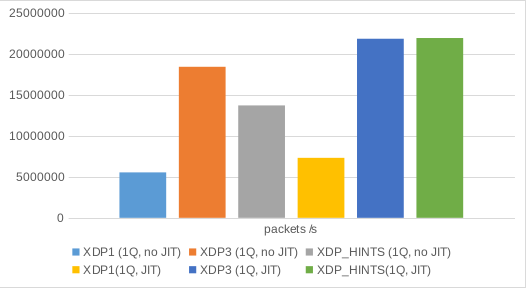
\includegraphics[width=3.31in]{xdp-programs-performance.png}
\caption{XDP With and Without HW Hints}
\label{xdp-performance}
\end{figure}

\subsection{Implementation Approach 1: Common Metadata Structure}

The most obvious approach to passing metadata through the xdp\_buff is to have a kernel structure that is defined to carry the data itself. This would be something each network driver would need to implement to translate HW offloads into the structure. While this would provide a vendor-agnostic solution to represent data, it imposes ABI restrictions to the XDP metadata core. Vendors would need to agree on this structure, and then this would become part of the UAPI, which means it cannot change once it is established, aside from additions. This rigidity of the interface, plus trying to have all vendors agree on a common structure to express specific hardware behaviors, is not a model believed to be sustainable moving forward.

\subsection{Implementation Approach 2: Vendor Logic in eBPF Libraries}

A different approach of processing metadata passed from a driver to the XDP core is to provide vendor-specific helper functions in the eBPF libraries in userspace. In this approach, a helper function such as bpf\_get\_hints() could then derive the underlying hardware, and call the vendor-specific hints-retrieval helper function. The main advantage to this approach is no kernel-level ABI is imposed through UAPI, so each vendor controls how the metadata is packed into the xdp\_buff. This approach can also provide a software fallback mechanism, in the case the underlying hardware doesn't provide the requested hints.
\newline
\indent However, the disadvantage to this approach is it requires eBPF and XDP programs to have knowledge of the underlying hardware they're running on. This introduces a requirement on XDP and eBPF that hasn't existed previously, where the program models avoided knowing or relying on specific hardware to operate.

\subsection{Implementation Approach 3: Chained XDP Programs With Helper Functions}

TBD

\section{Dynamic Programming of HW Hints}

TBD

\subsection{Using tc}

TBD

\subsection{Express Hints via eBPF Sections}

TBD

\subsection{XDP Per Queue}

TBD


\section{Conclusion}
Utilizing smarter network device offloads is going to be crucial in maximizing the performance and efficiency of XDP programs.  As these XDP programs become more and more complex with packet processing and parsing, the natural direction is to utilize network devices as they become smarter.  However, the expression of the hints from hardware, and programming of the underlying hardware to present the hints, is something the Linux kernel network community will need to work together on to best design a sustainable and scalable model.

\section{Acknowledgments}
We would like to acknowledge the NetDev 2.2 selection committee for inviting us to submit and present this paper.

\bibliographystyle{pj-netdev-2.2}
\bibliography{pj-netdev-2.2}

\section{Author Biographies}
Peter Waskiewicz Jr (PJ) is a Senior Linux Kernel Engineer in the Networking Division of Intel's Communications Group. He has maintained and helped create the igb, ixgbe, and i40e wired Ethernet network drivers, the initial Tx multiqueue support in the Linux kernel network stack, and added Data Center Bridging support to the Linux kernel. He also worked in Intel's Open Source Technology Center on the x86 kernel tree, enabling advanced features in the Broadwell and Skylake microarchitectures. Prior to returning to Intel, PJ was a Senior Principal Engineer at NetApp in the SolidFire division, where he was the chief Linux kernel and networking architect for the SolidFire scale-out cloud storage platform.
\newline
\newline
Anjali Singhai Jain is 
\newline
\newline
Neerav Parikh is
\newline
\newline
Parthasarathy Sarangam is

\end{document}
